\scanpage{84}
$\widetilde u\circ\widetilde{\alpha_i}$ un $\Delta$-foncteur s'exprime par la condition de rendre inversibles certaines flèches $\Sigma$ \deleted{dans}\inserted{de} $\widetilde D$ [du moins si \margin{\figure{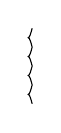
\begin{tikzpicture}\draw (0,0) sin (-.05,.12) cos (0,.24) sin (-.05,.36) cos (0,.48) sin (-.05,.60) cos (0,.72) sin (-.05,.84) cos (0,.96);\end{tikzpicture}}}on suppose que les $\Delta$-foncteurs sont définis par des prop. de commutation à certains types de $\underset{\leftrightarrow}{\lim}$ qui existent dans toutes les cat. éléments de $\Delta$]. Il n'est pas clair qu'on puisse se réduire au cas $\Sigma$ petit (si les $A_i$ \unsure{en|ne} sont petites\ldots, ce qui n'est \uline{guère} le cas que si les \unsure{p.quets|paquets|types} de diagrammes $d',d''$ par rapport auxquels on veut prendre des $\varprojlim$ et $\varinjlim$ et y commuter, sont petits) ; donc il faut alors travailler avec des sous-catégories ``génératrices'' petites, en un sens convenable\ldots.

Construction des 2-limites dans $(\mathrm{Cat})$ : elle est faite dans SGA 4 \uline{VI} en prenant la catégorie totale de la catégorie cofibrée envisagée et en rendant inversibles les morphismes cartésiens.

\medskip\hrule\medskip

``Théorie'' $T$ sur $\Delta$ : 2-catégorie cofibrée sur $\Delta$ i.e. 2-pseudofoncteur
\[
\Delta\xrightarrow{T}\mathrm{Cat}
\]
Ils forment une 2-catégorie
\[
\mathrm{Th\acute e}(\Delta)
\]
Dedans, on a
\[
\tau\in\mathrm{Ob}\,\mathrm{Th\acute e}(\Delta)\qquad \tau(C)=C
\]
On pose
\[
\underline{\mathrm{Hom}}_{\deleted{\unsure{\Delta}}}(T,\tau)=B_T\qquad
\text{catégorie \deleted{classifiante}\inserted{des constructions}}
\]
\uline{NB} Si $T$ est 2-représenté par $R\in\mathrm{Ob}\,\Delta$
\[
T(C)\simeq\underline{\mathrm{Hom}}_{\Delta}(R,C)
\]
alors on a \deleted{\unsure{Équiv|Équiv.}} pour tte théorie $T'$ sur $\Delta$
\[
\underline{\mathrm{Hom}}(T,T')\simeq T'(R)
\]
en particulier
\[
B_T=\underline{\mathrm{Hom}}(T,\tau)\simeq\tau(R)=R
\]
% archive sheet number: 83
